\section{Evaluation}
\label{sec:eval}

We evaluate retrieval, consolidation, the write and hook screens, and the vector index. Every number comes from the harness in the repository (\code{jevmem eval} and the scripts in \code{evals/}); a single live run per measurement; Jev is not perfectly deterministic, so differences under about 0.03 are noise. We do not re-measure \jevmempaper's LoCoMo question-answering accuracy: we measure whether the right \emph{note} reaches the agent, a different quantity.

\subsection{Datasets}

\begin{table*}[t]
\caption{Evaluation sets. ``Unans.'' = questions whose answer is not in memory (gold is empty).}
\label{tab:data}
\small
\begin{tabular}{@{}llll@{}}
\toprule
Set & Notes & Questions & Remark \\
\midrule
orbit & 25 & 30 (6 unans.) & in-sample tuning set \\
harbor & 40 & 41 (6 unans.) & held-out, run once with frozen defaults \\
LoCoMo c0--c9 & one per dialogue turn, sessions 1--4 & 45 (conv-26) + 272 (90 unans.) & adversarial questions with later evidence become unanswerable \\
SpaceMaker commits & 57 commit subjects & 31 (6 unans.) & private \\
srxy (commits + docs) & 138 & 47 (8 unans.) & private \\
\bottomrule
\end{tabular}
\end{table*}

The small sets were written by the author, the held-out set after the system existed, and most tuning data come from SpaceMaker. For LoCoMo~\cite{maharana2024locomo} we make one note per dialogue turn of sessions 1--4, stamped with the session date; adversarial questions whose evidence lies in later sessions become unanswerable. Metrics: \emph{recall} (fraction of gold notes returned), \emph{exact} (all gold notes returned), items and characters returned, latency, Jev calls and input tokens, and \emph{abstention} (\code{sufficient} is not true on an unanswerable question).

\subsection{Retrieval}

\begin{figure}[t]
\centering
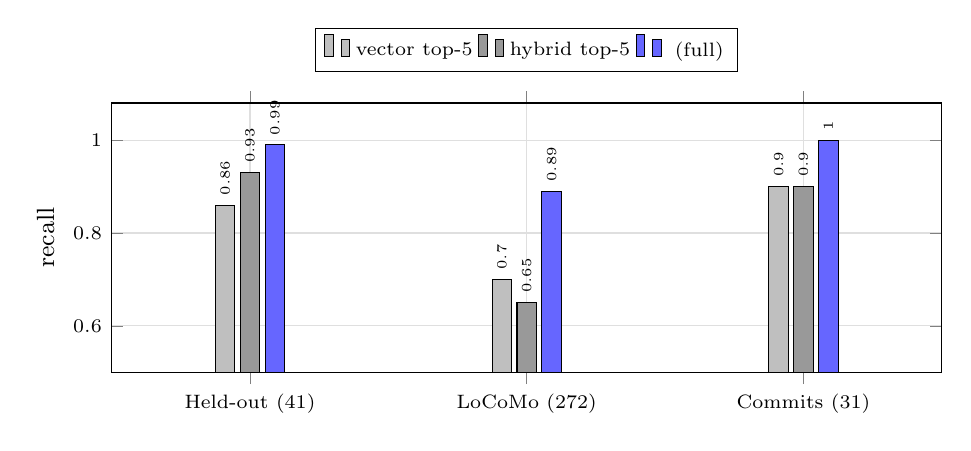
\begin{tikzpicture}
\begin{axis}[
  ybar, width=\columnwidth, height=5cm, bar width=7pt, ymin=0.5, ymax=1.08,
  symbolic x coords={Held-out (41),LoCoMo (272),Commits (31)}, xtick=data,
  ylabel={recall}, legend style={at={(0.5,1.28)},anchor=north,legend columns=-1,font=\scriptsize},
  tick label style={font=\scriptsize}, label style={font=\small}, enlarge x limits=0.25,
  nodes near coords, nodes near coords style={font=\tiny, rotate=90, anchor=west}, every node near coord/.append style={/pgf/number format/fixed, /pgf/number format/precision=2},
  grid=major, grid style={gray!25}]
\addplot[fill=gray!50] coordinates {(Held-out (41),0.86)(LoCoMo (272),0.70)(Commits (31),0.90)};
\addplot[fill=gray!80] coordinates {(Held-out (41),0.93)(LoCoMo (272),0.65)(Commits (31),0.90)};
\addplot[fill=blue!60] coordinates {(Held-out (41),0.99)(LoCoMo (272),0.89)(Commits (31),1.00)};
\legend{vector top-5, hybrid top-5, \jevmem{} (full)}
\end{axis}
\end{tikzpicture}
\caption{Recall of the gold note(s), \code{bge-small} embeddings. Baselines return five notes; \jevmem{} returns 1.4, 2.3 and 2.1 on average.}
\label{fig:recall-bars}
\end{figure}

Figure~\ref{fig:recall-bars} summarizes recall. On the held-out set \jevmem{} reaches 0.99 against 0.86 (vector) and 0.93 (hybrid); on pooled LoCoMo (9 conversations, 272 questions) 0.89 against 0.70 and 0.65; on SpaceMaker commit notes 1.00 against 0.90. Note that hybrid (BM25 $\oplus$ vector) is worse than vector on LoCoMo, where dialogue turns share vocabulary. At the same time \jevmem{} injects fewer notes: 1.4--2.3 instead of 5.

\begin{table}[h]
\caption{Pooled LoCoMo (272 questions), \code{bge-small}.}
\label{tab:locomo}
\small
\begin{tabular}{@{}lrrrrr@{}}
\toprule
Method & Recall & Items & Calls & Tokens & Latency \\
\midrule
vector top-5 & 0.70 & 5.0 & --- & --- & --- \\
hybrid top-5 & 0.65 & 5.0 & --- & --- & --- \\
lite & 0.84 & 3.0 & 1.0 & 2.1k & 0.25\,s \\
flat (no graph) & 0.85 & 1.6 & 4.0 & 3.8k & 0.94\,s \\
full & \textbf{0.89} & 2.3 & 5.9 & 9.5k & 1.44\,s \\
\bottomrule
\end{tabular}
\end{table}

\begin{table}[h]
\caption{Recall by question kind on pooled LoCoMo.}
\label{tab:kind}
\small
\begin{tabular}{@{}lrrrr@{}}
\toprule
Kind & $n$ & vector & lite & full \\
\midrule
single-hop & 102 & 0.70 & 0.87 & 0.92 \\
temporal & 48 & 0.81 & 0.90 & 0.94 \\
multi-hop & 19 & 0.60 & 0.76 & 0.82 \\
inference & 13 & 0.38 & 0.54 & 0.60 \\
\bottomrule
\end{tabular}
\end{table}

\paragraph{Where the graph helps.} On the single conversation conv-26, multi-hop recall rises from 0.20 (vector) to 0.70. On srxy, temporal questions score 0.04 (vector), 0.38 (lite) and 0.83 (full): the temporal graph and time-aware routing matter most for ``what did we decide \emph{before} X''. Honest counter-evidence: on srxy, graph expansion did not help (flat 0.93, full 0.92), and on pooled LoCoMo inference questions stay at 0.60.

\paragraph{Auto mode.} Pooled over 14 sets (466 questions), full reaches 0.910 recall at 10.4k tokens and 100\% escalation, lite 0.876 at 2.8k and 14\%, and the chosen \code{auto} setting (multi-hop $\ge 0.6$, temporal $\ge 0.8$) \textbf{0.911 at 6.3k tokens with 44\% escalation} (Figure~\ref{fig:tokens}). Dropping the temporal trigger cost srxy temporal recall (0.58 vs.\ 0.83); additionally escalating when lite says ``insufficient'' added 0.002 recall for 24\% more tokens and is off.

\begin{figure}[t]
\centering
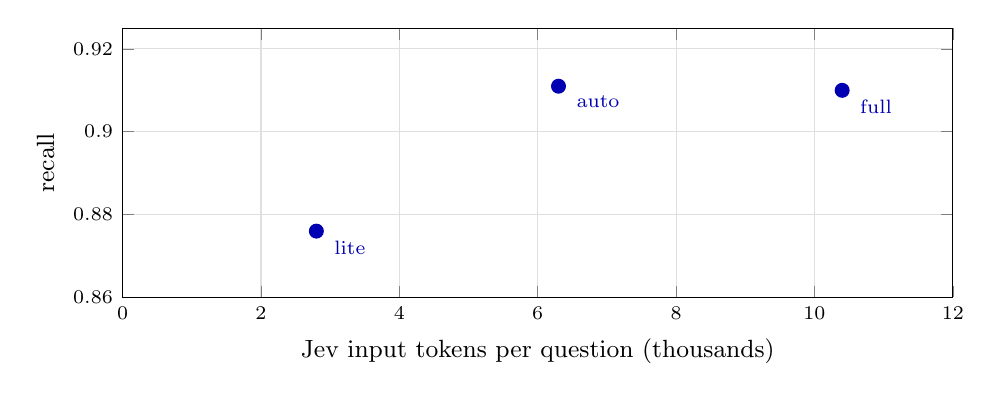
\begin{tikzpicture}
\begin{axis}[
  width=\columnwidth, height=5cm, xlabel={Jev input tokens per question (thousands)}, ylabel={recall},
  xmin=0, xmax=12, ymin=0.86, ymax=0.925, grid=major, grid style={gray!25},
  tick label style={font=\scriptsize}, label style={font=\small},
  nodes near coords, point meta=explicit symbolic, nodes near coords style={font=\scriptsize, anchor=north west, xshift=3pt}]
\addplot[only marks, mark=*, mark size=2.5pt, color=blue!70!black] coordinates {
 (2.8,0.876) [lite]
 (6.3,0.911) [auto]
 (10.4,0.910) [full]};
\end{axis}
\end{tikzpicture}
\caption{Cost--recall trade-off pooled over 14 sets (466 questions). Auto matches full recall for about 40\% fewer tokens.}
\label{fig:tokens}
\end{figure}

\subsection{Knowing what it does not know}

Because the agent is told to look elsewhere when memory is insufficient, abstention matters as much as recall. Full abstains on 85 of 90 unanswerable LoCoMo questions (94\%) and on all 6 of the SpaceMaker set; lite abstains on 94\% of 126 unanswerable questions pooled (97\% with the first thresholds, which flagged 11\% of answerable questions as insufficient; the chosen $0.3/0.7$ thresholds flag 4\%). The accuracy-optimal full-mode thresholds ($0.2$--$0.3/0.85$) score 0.89 against 0.85 for ours but let 9\% of unanswerable questions through instead of 5\%; leave-one-set-out accuracy is 0.88 either way, so we kept the defaults. The plain vector baselines can never abstain.

\subsection{Consolidation}

On labelled note pairs, each judged in both write orders (tuning 80 cases from 40 pairs, held-out 44 cases from 22 pairs): the original questions got 46/80 and 22/44 right; order-neutral questions got 79/80 and 43/44, and adding the ``reports a change'' question 80/80 and 44/44 with \textbf{no false flags on distinct pairs}. A fresh second held-out set (32 cases, 16 pairs) was 32/32. The new ``reports a change'' scores separate cleanly (superseded 0.68--0.97, others $\le 0.65$), as do coverage (duplicates $\ge 0.78$ both ways, subsumed $\ge 0.86$ one way, others $\le 0.42$) and pattern (repeated episodes 0.81--0.90, others $\le 0.59$). For same-timestamp ties, 32 of 36 became correctly superseded and all 18 true contradictions stayed \code{contradicts}. On SpaceMaker's live store, a full re-judge flagged exactly its three known stale notes (a fourth, a rename, later). The thresholds were tuned on the tuning set and checked on held-out sets; the pair sets are small.

\subsection{Write and hook screens}

\begin{table}[h]
\caption{Screens. ``Tune/holdout'' = threshold chosen on the first, checked on the second.}
\label{tab:screens}
\small
\begin{tabular}{@{}p{2.1cm}p{5.1cm}@{}}
\toprule
Screen & Result \\
\midrule
Injection & 0/15 benign blocked, 0/10 malicious missed (tuned on the same set: a regression test, not a rate) \\
Status ($\ge 0.85$) & 0 errors on tune (36) and holdout (24); status notes score $\ge 0.93$, others $\le 0.70$ \\
Auto-capture & 0 false captures on 123 real prompts (82 tune, 41 holdout); 11 of 12 synthetic standing rules stored \\
Prompt hook (needs-memory 0.20) & on-topic prompts with a gold note: 21/22; off-topic prompts with nothing injected: 19/22; 12/12 on the held-out prompts \\
Instruction-file skip & 19/23 restating notes by embedding alone; 22/23 with the borderline Jev band; 0 of 59 other notes skipped \\
\bottomrule
\end{tabular}
\end{table}

For SessionStart ranking over 31 sessions, hit@10 rises from 0.39 (no git context) to 0.52 (context weight 8). In a live session the instruction-file filter missed three paraphrases of a rule (coverage 0.30--0.43, below its threshold) while a non-restating note scored 0.49: no threshold separates them.

\subsection{Vector index}

At 100k notes (384-d, scoped top-10) the in-RAM matrix answers in 4.5\,ms (about 150\,MB), \code{sqlite-vec} in 12\,ms, LanceDB in 55--80\,ms. At one million notes (10 scopes, synthetic clustered vectors, 32 cores) the scoped p50 is 33\,ms for the matrix (1.5\,GB, exact), 44\,ms for \code{sqlite-vec}, 67\,ms for LanceDB IVF-PQ (recall 0.98), 3.5\,ms for a Qdrant server (0.996) and 3.3\,ms for pgvector HNSW with tuned parameters (0.975) but only 0.40 recall with defaults. A single developer's project stays far below 100k notes, so the default is exact search; the larger backends exist for shared stores.

\subsection{Threats to validity}

(1) \textbf{Small, author-written sets}: the held-out notes were written by the same person after the system existed. (2) \textbf{One run per measurement}; differences under 0.03 are noise. (3) \textbf{Tuning is dominated by SpaceMaker}; the hook and SessionStart weights come from 31 sessions and 44 prompts of one project. (4) \textbf{LoCoMo is conversational}; we convert turns to notes, which is not what our agents write. (5) \textbf{Unanswerable questions} are mostly adversarial in a style the model handles well. (6) \textbf{Vendor figures} (latency about 70--500\,ms per call, about \$0.042 per million input tokens) are quoted from the vendor and not independently measured. (7) The \textbf{field study} has one project, one developer and 12 days; it cannot show that the approach generalizes or measure the effect on agent task success.
